\documentclass[acmsmall]{acmart}
% clear acmtog.cls footer settings
\fancyfoot{}
\setcopyright{none}
\renewcommand\footnotetextcopyrightpermission[1]{}
\pagestyle{plain}
%remove reference format
\settopmatter{printacmref=false}
\numberwithin{figure}{subsection}
%
\usepackage{hyperref}
\usepackage{listings}
\usepackage{fancyvrb}
\usepackage{tikz} 

\DefineVerbatimEnvironment{code}{Verbatim}{fontsize=\small}
\begin{document}

\title{Core Documentation}

\author{Juvix Team}

\maketitle
\thispagestyle{empty}
\tableofcontents
\clearpage

\section{Pipeline}

\usetikzlibrary{fit}
\begin{tikzpicture}[node distance={14mm}, thick, main/.style = {draw, rectangle}] 
\node[main] (1) {Juvix source code}; 
\node[main] (2) [below of=1] {ML AST}; 
\node[main] (3) [below of=2] {S-expression AST}; 
\node[main] (4) [below of=3] {Desugared S-expression}; 
\node[main] (5) [below of=4] {Context of S-expression}; 
\node[main] (6) [below of=5] {Desugared Context of S-expression}; 
\node[main] (7) [below of=6] {Core HR}; 
\node[main] (8) [below of=7] {Core IR}; 
% TODO: From here, it's already type checked. Make it explicit
\node[main] (11) [below of=8] {Core Erased}; 
\node[main] (12) [below of=11] {Erased AnnTerm (with Return)}; 
\node[main] (13) [below of=12] {Erased AnnTerm (without Return)}; 
\node[main] (14) [below of=13] {Backend}; 
\draw[->] (1) -- node[midway, right] {\href{https://github.com/heliaxdev/juvix/blob/develop/library/Frontend/src/Juvix/Frontend/Parser.hs}{Frontend: Juvix.Frontend.Parser.hs (parse)}} (2); 
\draw[->] (2) -- node[midway, right] {\href{}{???}} (3); 
\draw[->] (3) -- node[midway, right] {\href{https://github.com/heliaxdev/juvix/blob/develop/library/Translate/src/Juvix/Desugar.hs}{Translate: Juvix.Desugar.hs (op)}} (4); 
\draw[->] (4) -- node[midway, right] {\href{https://github.com/heliaxdev/juvix/blob/develop/library/Translate/src/Juvix/Contextify.hs}{Translate: Juvix.Contextify.hs (contextify)}} (5); 
\draw[->] (5) -- node[midway, right] {\href{}{???}} (6); 
\draw[->] (6) -- node[midway, right] {\href{https://github.com/heliaxdev/juvix/blob/develop/library/Translate/src/Juvix/ToCore/FromFrontend.hs}{Translate: Juvix.ToCore.FromFrontend.hs}} (7); 
\draw[->] (7) -- node[midway, right] {\href{https://github.com/heliaxdev/juvix/blob/develop/library/Core/src/Juvix/Core/Translate.hs}{Core: Juvix.Core.Translate.hs (hrToIR)}} (8); 
\draw[->] (8) -- node[midway, right] {\href{https://github.com/heliaxdev/juvix/blob/develop/library/Core/src/Juvix/Core/Erasure/Algorithm.hs}{Core: Juvix.Core.Erasure.Algorithm.hs (erase)}} (11);
\draw[->] (11) -- node[midway, right] {\href{https://github.com/heliaxdev/juvix/blob/develop/library/Core/src/Juvix/Core/ErasedAnn/Conversion.hs}{Core: Juvix.Core.ErasedAnn.Conversion.hs (convertTerm)}} (12);
% TODO: Move toRaw to Erased module
\draw[->] (12) -- node[midway, right] {\href{}{Core: Juvix.Core.Pipeline.hs (toRaw)}} (13);
\draw[->] (13) -- node[midway, right] {\href{}{To Backend}} (14);
\node[draw,dotted,fit=(3) (4) (5) (6), label={[xshift=0mm]left:{S-expressions}}] {};
\node[draw,dotted,fit=(7) (8), label={[xshift=0mm]left:{Terms == Types}}] {};
\node[draw,dotted,fit=(11) (12) (13), label={[xshift=0mm]left:{Typechecked}}] {};

\end{tikzpicture} 

\section{HR}
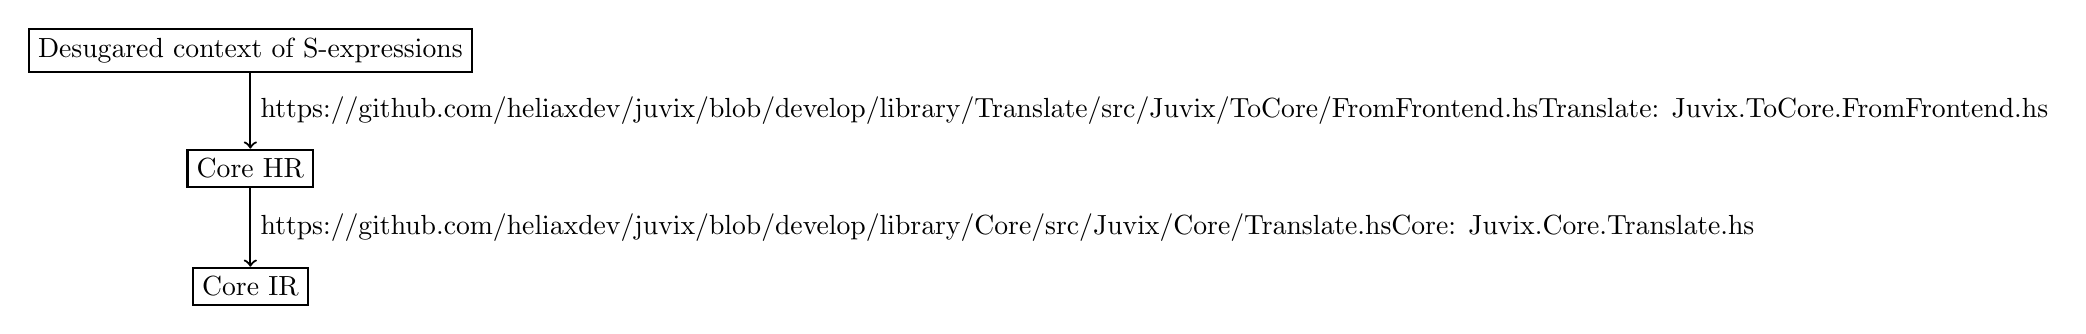
\begin{tikzpicture}[node distance={15mm}, thick, main/.style = {draw, rectangle}] 
\node[main] (1) {Desugared context of S-expressions}; 
\node[main] (2) [below of=1] {Core HR}; 
\node[main] (3) [below of=2] {Core IR}; 
\draw[->] (1) -- node[midway, right] {\href{https://github.com/heliaxdev/juvix/blob/develop/library/Translate/src/Juvix/ToCore/FromFrontend.hs}{Translate: Juvix.ToCore.FromFrontend.hs}} (2); 
\draw[->] (2) -- node[midway, right] {\href{https://github.com/heliaxdev/juvix/blob/develop/library/Core/src/Juvix/Core/Translate.hs}{Core: Juvix.Core.Translate.hs}} (3); 
\end{tikzpicture} 
% Relevant questions
% Why does it exist?
% Where is it placed in the pipeline?
% How is it used?
% How is the code in there?

HR stands for Human Readable.

This is a small module. It basically extends the Intermediate Representation (IR) base types to include names rather than De Bruijn indices.

As with any module in Juvix Core, an understanding of the \href{https://heliaxdev.github.io/extensible-data/Extensible.html}{extensible-data} library is required.

As mentioned, the goal is to use names instead of De Bruijn indices. Even though HR is a prior step in the pipeline than IR, the code is structured in a way that the \textit{base} types exist in IR and other modules \textit{extend} from it. These base types live in \href{https://github.com/heliaxdev/juvix/blob/develop/library/Core/src/Juvix/Core/IR/Types/Base.hs}{Juvix.Core.IR.Types.Base}. 
    
Do all types get affected by this distinction between HR and IR? No. Only \textit{binders} do. A binding is represented by an identifier. In the context of HR, this identifier is a name and this name is bound to a variable. Names must be unique. Binders in Juvix are:
\begin{enumerate}
    \item \textbf{Pi}

    A function whose type of return value varies with its argument is a dependent function and the type of this function is called \textit{pi-type}.
    
    Function types $(x \stackrel{\pi}{:} S) \rightarrow T$ record how the function will use its argument via the $\pi$ annotation.

    \begin{equation*}
       \dfrac{0\Gamma \vdash S \; 0 \Gamma, x \stackrel{0}{:} S \vdash T }{0 \Gamma \vdash (x \stackrel{\pi}{:} S) \rightarrow T} 
    \end{equation*}

    More details in \href{https://bentnib.org/quantitative-type-theory.pdf}{Syntax and Semantics of Quantitative Type Theory}.

    \bigskip

    We've encoded it in Juvix.Core.IR.Types.Base as follows:
    \begin{lstlisting}[language=haskell]
data Term primTy primVal = 
        ...
        | Pi Usage (Term primTy primVal) (Term primTy primVal)
        | ...
    \end{lstlisting}

    % TODO: Represent Pi in Juvix source code and its translation to HR and IR
    Here's an example of equivalent IR and HR Pi types:

    % TODO: Can we have a better example?
    \begin{lstlisting}[language=haskell]
        HR.Pi Usage.Omega "a" (HR.PrimTy ()) (HR.PrimTy ())
    \end{lstlisting}
    \begin{equation*}
      \Leftrightarrow  
    \end{equation*}
    \begin{lstlisting}[language=haskell]
        IR.Pi Usage.Omega (IR.PrimTy ()) (IR.PrimTy ())
    \end{lstlisting}
    \item \textbf{Lam}

    \begin{equation*}
       \dfrac{\Gamma, x \stackrel{\sigma \pi}{:} S \vdash M \stackrel{\sigma}{:} T }{\Gamma \vdash \lambda x \stackrel{\pi}{:} S .M^T \stackrel{\sigma}{:} (x \stackrel{\pi}{:} S) \rightarrow T} 
    \end{equation*}

    Forgetting the resource annotations, this is the standard introduction rule for dependent function types. We require that the abstracted variable $x$ has usage $\sigma \pi$ (multiplication by $\sigma$ is used to enforce the zero-needs-nothing).

    \begin{lstlisting}[language=haskell]
data Term primTy primVal = 
        ...
        | Lam (Term primTy primVal)
        | ...
    \end{lstlisting}


    Here's an example of equivalent IR and HR lambda types:

    \begin{lstlisting}[language=haskell]
        HR.Lam "x" (HR.Lam "y" (HR.Elim (HR.Var "x"))
    \end{lstlisting}
    \begin{equation*}
      \Leftrightarrow  
    \end{equation*}
    \begin{lstlisting}[language=haskell]
        IR.Lam (IR.Lam (IR.Elim (IR.Bound 1)))
    \end{lstlisting}

    \item \textbf{Sig}

    Sig stands for \textit{Sigma} type (not signature!), understood as existential quantifier. It is represented as $(x \stackrel{\pi}{:} S) \otimes T$. It captures the idea of an ordered pair where the type of the second term is dependent on the value of the first. For example, $\Sigma n : \mathbb{N}. \text{Vec A } n$ is actually equivalent to $List A$ because we can represent sequences of arbitrary length.

    \begin{equation*}
        \dfrac{0\Gamma \vdash A \; \; 0\Gamma, x \stackrel{0}{:} S \vdash T}{0\Gamma \vdash (x \stackrel{\pi}{:} S) \otimes T}
    \end{equation*}

    In a dependent pair ($\Sigma$) type, each half has its own usage. The \textit{usage} ($\pi$) of $Sig$ in the definition and in the following code refers to how many times the first argument may be used:

    \begin{lstlisting}[language=haskell]
data Term ty val = 
        ...
        | Sig Usage (Term ty val) (Term ty val)
        | ...
    \end{lstlisting}

    \item \textbf{Let}
    
    Some constructions allow the binding of a variable to a value. This is called a "let-binder". In a "let-binder", only once variable can be introduced at the same time.

    \begin{lstlisting}[language=haskell]
data Term ty val = 
        ...
        | Let Usage (Elim ty val) (Term ty val)
        | ...
    \end{lstlisting}
\end{enumerate}


The code representing the binders above are written in IR form.
The following code extends binder terms, using the \href{https://heliaxdev.github.io/extensible-data/Extensible.html}{extensible-data} library. The syntax of the type theory is defined by mutual induction between terms, with types specified in advance, and eliminations with types synthesized. This is why we need to extend $Elim$ as well.

\begin{lstlisting}[language=haskell]
extTerm :: p1 -> p2 -> IR.ExtTerm
extTerm =
  \_primTy _primVal ->
    IR.defaultExtTerm
      { IR.nameLam = "Lam0",
        IR.typeLam = Just [[t|NameSymbol.T|]],
        IR.namePi = "Pi0",
        IR.typePi = Just [[t|NameSymbol.T|]],
        IR.nameSig = "Sig0",
        IR.typeSig = Just [[t|NameSymbol.T|]],
        IR.nameLet = "Let0",
        IR.typeLet = Just [[t|NameSymbol.T|]]
      }
\end{lstlisting}

In the snippet above we are extending and renaming $Lam$, $Pi$, $Sig$ and $Let$ with an additional name represented as $NameSymbol$, which is just a type alias of $NonEmpty \; Symbol$ that encodes a qualified name.

We call this function in $Juvix.Core.HR.Types$ using the \textit{extendTerm} function generated by \textit{extensible} (see \href{https://heliaxdev.github.io/extensible-data/Extensible.html}{extensible-data})

\begin{lstlisting}[language=haskell]
extendTerm "Term" [] [t|T|] extTerm
\end{lstlisting}

We rename $Lam$ to $Lam0$, $Pi$ to $Pi0$, etc. for convenience. This way we can reorder the type parameters using \href{https://ghc.gitlab.haskell.org/ghc/doc/users_guide/exts/pattern_synonyms.html}{pattern synonyms} and only export these patterns from the library


\begin{lstlisting}[language=haskell]
pattern Pi pi x s t = Pi0 pi s t x
\end{lstlisting}

The same procedure follows for \textit{Elim}, although there are a few differences. The data constructors \textit{Bound} and \textit{Free} don't make sense in the context of HR. We want to introduce a new data constructor, \textit{Var}, that holds the qualified name (\textit{NameSymbol}) set by some binder.

\begin{lstlisting}[language=haskell]
extElim :: p1 -> p2 -> IR.ExtElim
extElim =
  \_primTy _primVal ->
    IR.defaultExtElim
      { IR.typeBound = Nothing,
        IR.typeFree = Nothing,
        -- | Extend with extra constructor Var 
        -- that was not existing before
        IR.typeElimX = [("Var", [[t|NameSymbol.T|]])]
      }
\end{lstlisting}

% TODO: Explain patterns as well

\begin{lstlisting}[language=haskell]
extPattern :: p1 -> p2 -> IR.ExtPattern
extPattern =
  \_primTy _primVal ->
    IR.defaultExtPattern
      { IR.typePVar = Nothing,
        IR.typePatternX = [("PVar", [[t|NameSymbol.T|]])]
      }
\end{lstlisting}

\section{Erased}


Erased doesn't extend from IR types any more, but from its own types file. In contrast to previous steps in the pipeline, it distinguishes between terms and types.

At this point, terms have already been typechecked.

\subsection{ErasedAnn}

We retrieve the usage of a term and annotate the term with it. Certain backends can use the knowledge of a usage's term to optimise their compilation.

\end{document}